\section{Evaluation Design and Audited Model Results}
\label{sec:evaluation}

The evaluation reports four kinds of output: agreement with filing-derived labels, performance against development labels, comparison with historical human ratings, and saved company scores. Final values come from the consolidated audit and recovered-result JSON files. Each comparison records the dataset, reference source, and unit of analysis.

\subsection{Data groups, evaluation measures, and uncertainty}

For principle classification, Top-1 agreement is the share of passages whose highest-ranked principle matches the recorded label. Top-2 agreement is the share whose recorded label appears among the two highest-ranked principles. Top-2 gives an analyst a short candidate list. A higher Top-2 value does not mean better accuracy when only one answer is allowed.

Precision shows how reliable a predicted category is. If 100 passages receive an environmental-principle prediction and 90 carry that reference label, precision is 90\%. Recall shows how much of a reference category is found. If 100 passages carry the environmental label and the classifier finds 80, recall is 80\%. F1 balances precision and recall through the harmonic mean:
\begin{equation}
F1_k=\frac{2P_kR_k}{P_k+R_k},\qquad
\operatorname{MacroF1}=\frac{1}{9}\sum_{k=1}^{9}F1_k.
\label{eq:f1}
\end{equation}
Macro-F1 gives each principle equal weight, so the largest class cannot determine the entire score. Support means the number of reference examples for a principle. The references are weak labels. A result described as correct therefore means agreement with the recorded assignment, not an independent judgement of the passage's meaning.

A 95\% confidence interval shows uncertainty in an estimate under the stated sampling method. For classification and mapping, the audit uses 2,000 bootstrap samples with seed 4206. Companies are sampled with replacement, and all passages from a selected CIN are kept together. This CIN-cluster method accounts for passages from the same company being related. Paired comparisons use the same sampled companies for both methods. These intervals describe variation within the available data; label errors and earlier exposure during model development remain outside that estimate. The 20-company score comparison uses 10,000 bootstrap samples of company-score pairs with seed 42. No detector intervals were calculated.

\subsection{Method comparisons and generalisation checks}
\label{sec:comparison_summary}

Table~\ref{tab:comparison_summary} summarises three comparisons: results by label source, performance on concepts excluded from training, and supervised versus zero-shot mapping. The table records the examples and training conditions for each comparison. These are method and data-split comparisons rather than a controlled change to one component.

\begin{table}[tbp]
\centering\small
\caption{Three comparisons of Top-1 agreement with filing-derived labels. Data and training conditions are recorded for each row. Percentages from different rows describe different groups. Sections~\ref{sec:eval_sources}, \ref{sec:concept_diagnostics}, and~\ref{sec:eval_mapping} give intervals and further measures.}
\label{tab:comparison_summary}
\begin{tabularx}{\linewidth}{@{}L{2.6cm}L{2.5cm}L{3.1cm}Y@{}}
\toprule\textbf{Comparison} & \textbf{Evaluation population} & \textbf{Top-1 agreement} & \textbf{Interpretation}\\\midrule
Label source & B: 352; C: 5,364; notes: 485 segments & B: 63.35\%; C: 95.15\%; notes: 90.72\% & Results for parts of the same 6,201-row test set. Sources use different text and labelling rules.\\
Full-concept and excluded-concept training & Same 1,190 segments from 174 companies & Full concept: 97.98\%; excluded concept: 87.31\% & The training sets differ in concept coverage, example count, and seed.\\
Zero-shot MPNet versus supervised BERT & Same 6,201 segments from 175 companies & MPNet: 67.63\%; BERT: 93.00\% & The methods have different access to labels. The BERT value reuses the classifier result.\\\bottomrule
\end{tabularx}
\end{table}

The reported comparisons use the final labelled split and the training conditions listed in the table. Domain adaptation is part of the final model's training sequence. No separate numerical gain is assigned to adaptation or data cleaning.

\subsection{Dataset size and results by label source}
\label{sec:eval_sources}

The final single-label dataset contains 42,409 samples: 2,479 from explicit principle-axis facts, 36,513 from Section C mappings, and 3,417 from principle notes. The builder excludes 36,491 noisy facts and removes 2,640 groups with several labels. Fact rows and groups are different counting units. These exclusions cannot simply be added as final examples.

The Section B build starts with 41,898 narrative candidates. The content filter removes 16,684 candidates, leaving 25,214 clean entries. Removing 18 repeated same-label entries and 22,717 entries from groups with several labels produces 2,479 final rows. These steps reconcile the current source counts.

\begin{table}[tbp]
\centering\small
\caption{Final weak-label dataset by principle. The last column gives example counts in the company-separated test set.}
\label{tab:class_counts}
\begin{tabularx}{\linewidth}{@{}Yr r@{}}
\toprule\textbf{Principle} & \textbf{Dataset rows} & \textbf{Test rows}\\\midrule
P1: Ethics and governance & 5,015 & 773\\
P2: Sustainable goods and services & 5,566 & 808\\
P3: Employee and worker wellbeing & 11,835 & 1,715\\
P4: Stakeholder interests & 3,128 & 469\\
P5: Human rights & 3,095 & 449\\
P6: Environmental responsibility & 5,749 & 823\\
P7: Public policy advocacy & 543 & 69\\
P8: Inclusive growth & 2,475 & 368\\
P9: Consumer responsibility & 5,003 & 727\\\midrule
\textbf{Total} & \textbf{42,409} & \textbf{6,201}\\\bottomrule
\end{tabularx}
\end{table}

\begin{table}[tbp]
\centering\small
\caption{Recovered classifier results by label source on the same test set. A company can supply several sources, so the company counts overlap. Top-1 intervals are calculated by resampling companies.}
\label{tab:source}
\begin{tabularx}{\linewidth}{@{}Yrrrrl@{}}
\toprule\textbf{Source} & \textbf{Segments} & \textbf{CINs} & \textbf{Top-1} & \textbf{Top-2} & \textbf{Top-1 95\% CI}\\\midrule
Section B: explicit axis & 352 & 71 & 63.35\% & 80.40\% & 56.55--69.67\%\\
Section C: concept map & 5,364 & 174 & 95.15\% & 99.01\% & 94.41--95.92\%\\
Principle notes & 485 & 103 & 90.72\% & 95.46\% & 86.55--94.09\%\\\bottomrule
\end{tabularx}
\end{table}

Table~\ref{tab:source} reports agreement of 63.35\% for explicit-axis passages and 95.15\% for concept-mapped passages. Section C supplies 86.1\% of the full labelled dataset and 5,364 of the 6,201 test rows. The overall value therefore reflects the source mix. Section B contains the examples retained by the single-label filtering procedure. Figure~\ref{fig:source} presents the three sources together, and the excluded-concept tests provide a second view of performance across reporting questions.

\begin{figure}[tbp]
\centering
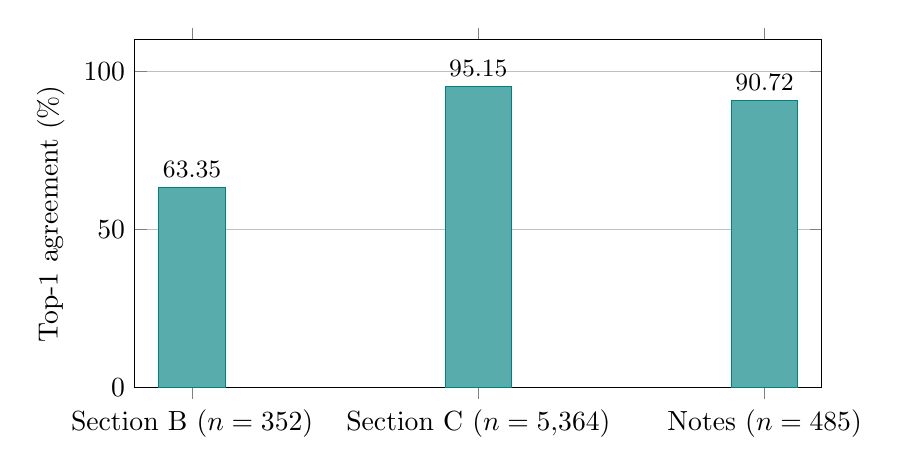
\begin{tikzpicture}
\begin{axis}[width=0.85\linewidth,height=6cm,ybar,bar width=24pt,
  ylabel={Top-1 agreement (\%)},ymin=0,ymax=110,
  symbolic x coords={B,C,Notes},xtick=data,
  xticklabels={Section B ($n=352$),Section C ($n=5{,}364$),Notes ($n=485$)},
  ymajorgrids=true,nodes near coords,nodes near coords style={font=\small},
  point meta=explicit symbolic]
\addplot[fill=teal!65,draw=teal] coordinates {(B,63.35) [63.35] (C,95.15) [95.15] (Notes,90.72) [90.72]};
\end{axis}
\end{tikzpicture}
\caption{Principle-label agreement by source. The bars compare explicitly tagged passages, concept-mapped passages, and principle notes using the filing-derived reference labels. Table~\ref{tab:source} gives confidence intervals calculated by resampling companies.}
\label{fig:source}
\end{figure}


\subsection{Recovered classifier performance and training history}

The recovered seed-99 model matches 5,767 of 6,201 reference labels. Top-1 agreement is 93.00\% (95\% CI: 92.04--93.89\%). The reference label appears among the two highest predictions for 6,057 examples, giving 97.68\% Top-2 agreement (95\% CI: 97.10--98.21\%). Macro-F1 is 0.9158 (95\% CI: 0.9036--0.9277). The text-overlap check identifies 50 exact train/test matches across different companies, or 0.81\% of test rows. The supervised split has zero CIN overlap.

Figure~\ref{fig:training} shows the five recorded epochs for seed 99. Validation macro-F1 rises from 0.9048 at epoch 1 to 0.9194 at epoch 4, then reaches 0.9189 at epoch 5. Validation loss rises over the same period. F1 describes category decisions, while loss also considers prediction confidence. The recorded selection criterion chooses epoch 4 by validation macro-F1.

\begin{figure}[tbp]
\centering
\begin{subfigure}{0.48\linewidth}
\centering
\begin{tikzpicture}
\begin{axis}[width=\linewidth,height=5.4cm,xlabel={Completed epoch},ylabel={Validation macro-F1},
  xmin=0.7,xmax=5.3,ymin=0.895,ymax=0.925,xtick={1,2,3,4,5},ymajorgrids=true,
  scaled y ticks=false,yticklabel style={/pgf/number format/fixed,/pgf/number format/precision=3}]
\addplot[teal,thick,mark=*] coordinates {(1,0.904818)(2,0.907187)(3,0.913640)(4,0.919368)(5,0.918854)};
\addplot[warm,only marks,mark=*,mark size=3.5pt] coordinates {(4,0.919368)};
\end{axis}
\end{tikzpicture}
\caption{Category agreement is highest at epoch 4.}
\end{subfigure}\hfill
\begin{subfigure}{0.48\linewidth}
\centering
\begin{tikzpicture}
\begin{axis}[width=\linewidth,height=5.4cm,xlabel={Completed epoch},ylabel={Validation loss},
  xmin=0.7,xmax=5.3,ymin=0.25,ymax=0.50,xtick={1,2,3,4,5},ymajorgrids=true]
\addplot[ink,thick,mark=square*] coordinates {(1,0.310062)(2,0.360093)(3,0.401145)(4,0.447556)(5,0.468024)};
\end{axis}
\end{tikzpicture}
\caption{Loss records changes in prediction confidence.}
\end{subfigure}
\caption{Five recorded training epochs for seed 99. The marked point identifies checkpoint 7,460, selected by validation macro-F1. The two panels present category agreement and probability-based loss, showing the recorded basis for checkpoint selection.}
\label{fig:training}
\end{figure}


Table~\ref{tab:per_principle} groups performance by principle; Table~\ref{tab:source} groups performance by label source. Each principle row shows prediction reliability, reference-category coverage, and the balance between both. P7 has only 69 test examples, so the P7 estimate needs extra care. Figure~\ref{fig:per_principle} summarises F1, while the table also gives precision, recall, and example counts.

\begin{table}[tbp]
\centering\small
\caption{Results for nine principles on 6,201 passages. Precision shows how often a predicted principle matches the reference. Recall shows how much of the reference category is found. F1 balances both.}
\label{tab:per_principle}
\begin{tabularx}{\linewidth}{@{}Yrrrr@{}}
\toprule\textbf{Principle} & \textbf{Support} & \textbf{Precision} & \textbf{Recall} & \textbf{F1}\\\midrule
P1: Ethics and governance & 773 & 0.9592 & 0.9431 & 0.9511 \\
P2: Sustainable goods and services & 808 & 0.9154 & 0.8837 & 0.8992 \\
P3: Employee and worker wellbeing & 1,715 & 0.9533 & 0.9644 & 0.9588 \\
P4: Stakeholder interests & 469 & 0.9611 & 0.9488 & 0.9549 \\
P5: Human rights & 449 & 0.9009 & 0.8508 & 0.8751 \\
P6: Environmental responsibility & 823 & 0.8943 & 0.9356 & 0.9145 \\
P7: Public policy advocacy & 69 & 0.8551 & 0.8551 & 0.8551 \\
P8: Inclusive growth & 368 & 0.8921 & 0.9212 & 0.9064 \\
P9: Consumer responsibility & 727 & 0.9259 & 0.9285 & 0.9272 \\
\midrule
Macro average & 6,201 & 0.9175 & 0.9146 & 0.9158\\\bottomrule
\end{tabularx}
\end{table}

\begin{figure}[tbp]
\centering
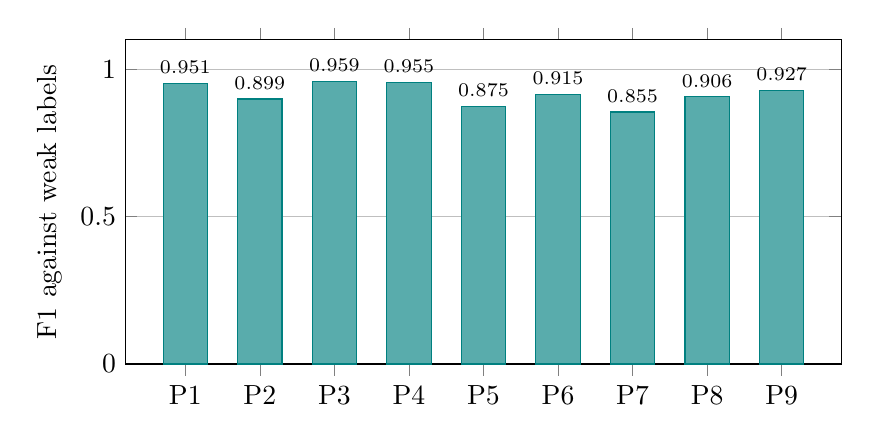
\begin{tikzpicture}
\begin{axis}[width=0.88\linewidth,height=5.7cm,ybar,bar width=16pt,ymin=0,ymax=1.10,
  ylabel={F1 against weak labels},symbolic x coords={P1,P2,P3,P4,P5,P6,P7,P8,P9},xtick=data,
  ymajorgrids=true,nodes near coords,nodes near coords style={font=\scriptsize,/pgf/number format/fixed,/pgf/number format/precision=3}]
\addplot[fill=teal!65,draw=teal] coordinates {(P1,0.9511)(P2,0.8992)(P3,0.9588)(P4,0.9549)(P5,0.8751)(P6,0.9145)(P7,0.8551)(P8,0.9064)(P9,0.9272)};
\end{axis}
\end{tikzpicture}
\caption{F1 by principle for the recovered classifier. A higher bar means a better balance of precision and recall against the recorded weak labels. P7 has 69 test examples, compared with 1,715 for P3. Table~\ref{tab:per_principle} gives all example counts and measures.}
\label{fig:per_principle}
\end{figure}


\subsection{Tests on excluded concepts and multiple labels}
\label{sec:concept_diagnostics}

Separating companies asks whether the model can classify passages from another company. Separating concepts asks whether the model can classify passages for reporting questions excluded from labelled training. The first check excludes 17 Section C concepts and evaluates 1,190 rows. On these same rows, the full-concept model reaches 97.98\% Top-1 agreement and the excluded-concept model reaches 87.31\%. The paired difference is $-10.67$ percentage points (95\% CI: $-12.36$ to $-8.96$). Both checkpoints passed strict parameter-name recovery before re-evaluation.

The full-concept model uses seed 99. The excluded-concept model uses seed 42 and fewer training examples. The paired interval describes the difference on shared test rows under these training conditions. The comparison includes changes in concept coverage, training examples, and seed.

Across three excluded-concept runs, mean Top-1 agreement is 81.64\%, with sample standard deviation 4.92 percentage points. Mean Top-2 is 95.34\%, with standard deviation 1.31 percentage points. Mean macro-F1 is 0.6752, with standard deviation 0.0170. Figure~\ref{fig:concept} shows each run and test size. Standard deviations describe variation across the three runs. All runs reuse the original test-company group, and concept exclusion is defined for labelled training. The earlier adaptation-corpus membership is described in Section~\ref{sec:classifier}.

\begin{figure}[tbp]
\centering
\begin{tikzpicture}
\begin{axis}[width=0.90\linewidth,height=6.2cm,ybar,bar width=17pt,ymin=0,ymax=112,
  ylabel={Top-1 agreement (\%)},symbolic x coords={H42,H17,H73},xtick=data,
  xticklabels={Test 42 ($n=1{,}190$),Test 17 ($n=1{,}167$),Test 73 ($n=1{,}169$)},
  ymajorgrids=true,legend style={at={(0.5,1.04)},anchor=south,legend columns=2},
  nodes near coords,nodes near coords style={font=\scriptsize,/pgf/number format/fixed,/pgf/number format/precision=2}]
\addplot[fill=ink!35,draw=ink] coordinates {(H42,97.98)(H17,96.06)(H73,97.18)};
\addlegendentry{Full-concept model}
\addplot[fill=teal!65,draw=teal] coordinates {(H42,87.31)(H17,79.18)(H73,78.44)};
\addlegendentry{Excluded-concept model}
\end{axis}
\end{tikzpicture}
\caption{Full-concept and excluded-concept training on three shared test groups. The tests contain 174, 173, and 174 companies from the original split. Excluded-concept mean agreement is 81.64\%, with sample standard deviation 4.92 percentage points across runs. Training examples and seeds are described in Section~\ref{sec:concept_diagnostics}; the standard deviation summarises variation across these runs.}
\label{fig:concept}
\end{figure}


The multi-label version groups company text and combines the recorded principle labels for each group. The test set contains 5,934 examples from the same 175 companies. Hit@1 checks whether the highest-ranked prediction belongs to the recorded label set and reaches 93.36\% (95\% CI: 92.54--94.11\%). At threshold 0.5, micro-F1 is 0.8898 (0.8743--0.9035), and macro-F1 is 0.8782 (0.8606--0.8942). The single-label model reaches Hit@1 of 93.55\% on the same grouped labels. This comparison evaluates an alternative target definition: one company-text example can contain several principle assignments, including assignments from generic text reused under different questions.

\subsection{Frozen text-vagueness results}

Table~\ref{tab:detector} reports the fixed detector on two separate groups. Batches 1 and 2 contain 80 earlier development examples. The detector flags 41 examples, and 29 flags match the reference vagueness label. The detector finds 29 of the 37 reference-vague examples. These counts give precision 0.7073 and recall 0.7838. In total, 60 of the 80 decisions match the reference, giving accuracy 0.7500 and F1 0.7436.

Batch 3 contains 70 AI-labelled examples. The detector flags 35 passages, and 21 flags match the AI vagueness label. The detector identifies 21 of the 26 passages labelled vague, giving F1 0.6885. Figure~\ref{fig:detector} displays precision, recall, and F1 alongside the 80-example development group. The groups use different passages and reference sources and are reported separately.

\begin{table}[tbp]
\centering\small
\caption{Fixed text-vagueness detector on two label groups. The first row uses 80 development examples, and the second uses 70 AI-labelled examples. Reference conditions are stated in the evaluation text.}
\label{tab:detector}
\begin{tabularx}{\linewidth}{@{}Yrrrrr@{}}
\toprule\textbf{Reference labels} & \textbf{N} & \textbf{Accuracy} & \textbf{Precision} & \textbf{Recall} & \textbf{F1}\\\midrule
Historical development labels & 80 & 0.7500 & 0.7073 & 0.7838 & 0.7436\\
AI annotations & 70 & 0.7286 & 0.6000 & 0.8077 & 0.6885\\\bottomrule
\end{tabularx}
\end{table}

\begin{figure}[tbp]
\centering
\begin{tikzpicture}
\begin{axis}[width=0.85\linewidth,height=6cm,ybar,bar width=17pt,ymin=0,ymax=1.12,
  ylabel={Decision measure},symbolic x coords={Precision,Recall,F1},xtick=data,
  ymajorgrids=true,legend style={at={(0.5,1.03)},anchor=south,legend columns=1},
  nodes near coords,nodes near coords style={font=\scriptsize,/pgf/number format/fixed,/pgf/number format/precision=3}]
\addplot[fill=ink!35,draw=ink] coordinates {(Precision,0.7073)(Recall,0.7838)(F1,0.7436)};
\addlegendentry{Development reference ($n=80$)}
\addplot[fill=teal!65,draw=teal] coordinates {(Precision,0.6000)(Recall,0.8077)(F1,0.6885)};
\addlegendentry{AI reference ($n=70$, exploratory)}
\end{axis}
\end{tikzpicture}
\caption{Precision, recall, and F1 for the fixed language detector. The first group contains 80 development examples; the second contains 70 AI-labelled examples. Precision describes how often a flag matches the reference, recall describes how many reference-vague passages are found, and F1 balances both. These measures cover the language branch.}
\label{fig:detector}
\end{figure}


The reported precision, recall, and F1 cover the combined word-list and sentence-similarity detector. Claim--figure and assurance-gap outputs are rule-generated review records without a completed accuracy evaluation. Batches 1 and 2 are development data, and annotation blinding is not documented in the saved records. Batch 3 uses one AI-generated annotation set and is an exploratory reference comparison. Continuous-score ROC AUC and between-rater agreement are outside the reported measures.

\subsection{Supervised transfer versus zero-shot mapping}
\label{sec:eval_mapping}

Both methods rank principles for the same 6,201 test examples. The MPNet definition-plus-anchor method reaches 67.63\% Top-1 and 83.34\% Top-2 agreement. The recovered supervised classifier reaches 93.00\% and 97.68\%. Table~\ref{tab:mapping} gives the confidence intervals. The paired Top-1 difference is $+25.37$ percentage points (95\% CI: $+24.02$ to $+26.71$). The comparison combines model representation and access to labelled training. The output measures principle-label agreement.

\begin{table}[tbp]
\centering\small
\caption{Principle mapping on the same company-separated test rows. Intervals resample companies. The supervised row reuses the classifier result and is not a second independent test.}
\label{tab:mapping}
\begin{tabularx}{\linewidth}{@{}Yrrl@{}}
\toprule\textbf{Method} & \textbf{Top-1} & \textbf{Top-2} & \textbf{Macro-F1}\\\midrule
MPNet zero-shot hybrid & 67.63\% & 83.34\% & 0.6405\\
\quad 95\% interval & 66.45--68.93\% & 82.31--84.38\% & 0.6248--0.6567\\
Recovered supervised transfer & 93.00\% & 97.68\% & 0.9158\\
\quad 95\% interval & 92.04--93.89\% & 97.10--98.21\% & 0.9036--0.9277\\\bottomrule
\end{tabularx}
\end{table}

The supervised row reuses the classifier evaluation from the same company-separated test set. Both methods are compared against the filing-derived reference labels defined in Section~\ref{sec:labels}. The result is reported once as an underlying model evaluation and reused for the mapping application.

\subsection{Transparency Score compared with historical human ratings}

The historical human-rating group contains 20 companies. Pearson correlation measures how automated and human scores vary together: $r=0.6314$ (95\% CI: 0.2683--0.8519; $p=0.0028$). Spearman correlation compares score ranks: $\rho=0.6285$ (95\% CI: 0.2321--0.8540). Mean absolute error is 12.16 points, and root mean squared error, which gives larger errors more weight, is 15.19 points. The audit reports $r^2=0.3986$. This squared correlation describes association; no separate predictive regression was fitted for this result.

The historical comparison uses 20 company ratings from one documented source. The saved file contains both ratings and automated scores; rater blinding is not documented. The original Zensar text packet includes a URL-related extraction issue, and Geojit's business model differs from manufacturing-oriented reporting items. Both companies remain in the full group. The analysis uses the original ratings and fixed score formula, with all 20 cases retained; synthetic ratings and AI assessments are kept separate.

\subsection{Checking the API connection}

The audit records a successful principle-mapping API request for 360 ONE WAM LIMITED on 19 October 2026. The response identifies the recovered seed-99 classifier and checkpoint path. The returned 89.17\% summary is the average model probability for that filing. This request verifies model loading for one company.

\FloatBarrier
